\documentclass[10pt]{article}
\usepackage{homework-style}

\begin{document}
\dz{6}
\date{21 декабря 2024}

\begin{tasks}
    \item Давным-давно барон Мюнхгаузен свои владения обнёс забором и нарисовал на карте. Забор изображён замкнутой несамопересекающейся ломаной, внутри которой — владения барона. Барон забыл, входит ли в его владения деревня Гаузеновка. Он смог найти лишь обрывок карты, на который попали его дом, деревня Гаузеновка и часть забора, проходящая по этому участку. Как узнать, входит ли деревня во владения барона?
    
    \begin{figure}[ht]
        \centering
        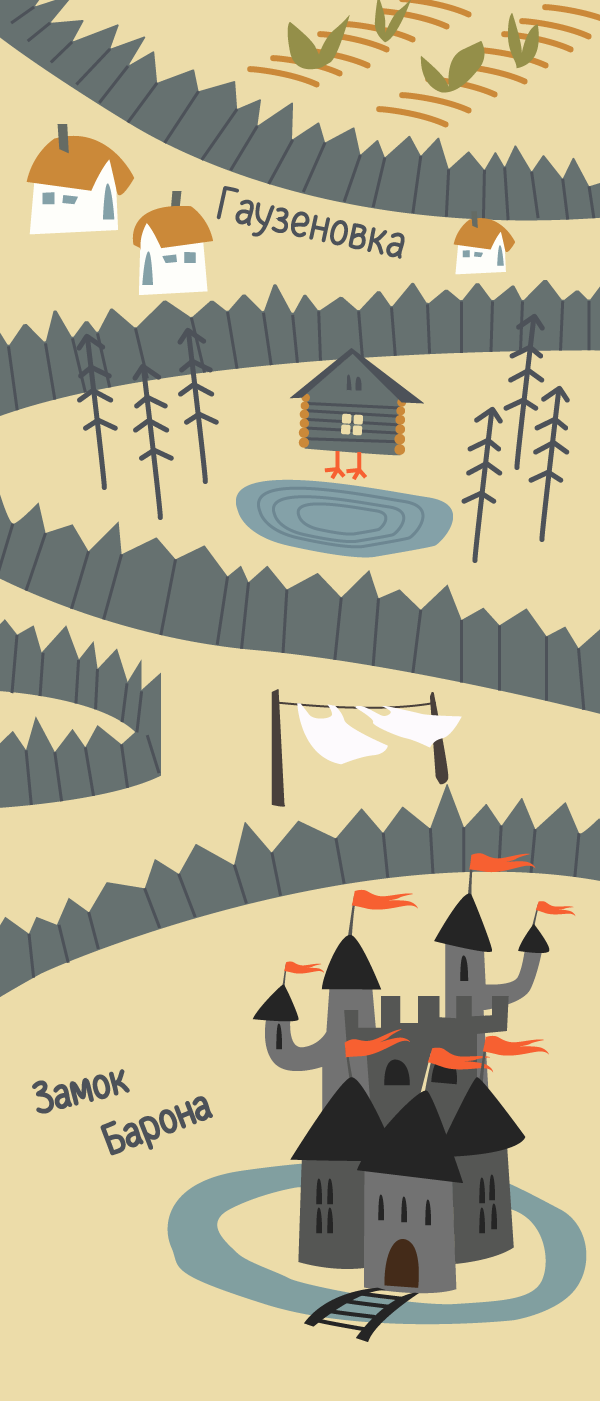
\includegraphics[width=0.25\linewidth]{картинка 7_Монтажная область 1.png}
    \end{figure}
    
    Постарайтесь как можно точнее сформулировать топологическое условие. Строгое доказательство не требуется.

    \begin{proof}
        [Решение]
        Представим себе путь из дома в деревню. Это будет какая-то непрерывная кривая. Таких путей, бесконечно много. Выберем какой-нибудь один такой путь, который будет лежать в нашей ``области видимости''.
        
        Пересекая забор мы меняем свою область с ``во владениях'' на ``вне владений'' и наоборот. Значит нам нужно лишь понять сколько раз по пути из дома до деревни Гаузеновка мы пересакаем забор. В данном случае это 3 раза (5 раз), т.е. мы будем вне владений, значит не лежит.
    \end{proof}

    \item Рассмотрим три следующих функции\footnote{Такие функции называются метриками Минковсого.} от пар точек на плоскости $\R^2$:
        \begin{itemize}
            \item $\rho_1((x,y), (x',y')) = |x-x'|+|y-y'|$;
            \item $\rho_2((x,y), (x',y')) = \sqrt{(x-x')^2+(y-y')^2}$;
            \item $\rho_\infty((x,y), (x',y')) = \max(|x-x'|, |y-y'|).$
        \end{itemize}
    Докажите, что каждая из этих функций задает метрику на плоскости. Нарисуйте в каждой из этих метрик шар радиуса 1 с центром в начале координат.
    \begin{proof}
        [Решение]
        Здесь нужно просто попроверять свойства метрики.
        \begin{conditions}
            \item Проверим для $\rho_1$: \begin{conditions}
                \item \textit{аксиома тождества:}\begin{align*}
                    \rho_1((x,y), (x',y')) = |x-x'|+|y-y'| = 0 \ifandonly\\\ifandonly \begin{cases}
                        |x-x'| = 0\\
                        |y-y'| = 0
                    \end{cases} \ifandonly (x, y) = (x', y').
                \end{align*}
                \item \textit{аксиома симметричности:}
                \begin{align*}
                    \rho_1((x,y),(x',y')) = |x-x'|+|y-y'| =\\= |x'-x|+|y'-y| = \rho_1((x',y'),(x,y)).
                \end{align*}
                \item \textit{неравенство треугольника:}
                \begin{align*}
                    &\rho_1((x_1,x_2),(y_1,y_2)) + \rho_1((y_1, y_2),(z_1, z_2)) =\\
                    &= |x_1-y_1|+|x_2-y_2| + |y_1-z_1|+|y_2-z_2| = \\
                    &= (|x_1-y_1|+ |y_1-z_1|)+(|x_2-y_2| +|y_2-z_2|) \geqslant \\
                    &\geqslant |x_1-y_1+y_1-z_1|+|x_2-y_2+y_2-z_2| = \\
                    &=|x_1-z_1|+|x_2-z_2| = \rho_1((x_1, x_2), (z_1,z_2)).
                \end{align*}
            \end{conditions}
            Значит функция $\rho_1$ действительно задает метрику на $\R_2$. 
            
            \begin{figure}[ht]
                \centering
                \begin{asy}
                    size(4cm); // Size of the graph
                    defaultpen(fontsize(8pt));
                    
                    real xmin = -4, xmax = 4, ymin = -4, ymax = 4;
                    
                    // Add grid lines (vertical and horizontal)
                    for (real i = floor(xmin); i <= ceil(xmax); ++i) if (i != 0){
                      draw((i, ymin) -- (i, ymax), gray(0.7));  // Vertical grid lines
                    }
                    for (real j = floor(ymin); j <= ceil(ymax); ++j) if (j != 0){
                      draw((xmin, j) -- (xmax, j), gray(0.7));  // Horizontal grid lines
                    }
                    
                    // Draw the axes
                    xaxis(xmin-.5, xmax+.5, arrow=Arrow(arrowhead=DefaultHead, size=1mm)); 
                    yaxis(ymin-.5, ymax+.5, arrow=Arrow(arrowhead=DefaultHead, size=1mm));
                    
                    // Define the vertices of the rhombus
                    pair A = (0, 3);
                    pair B = (-3, 0);
                    pair C = (0, -3);
                    pair D = (3, 0);
                    
                    // Fill and draw the rhombus
                    filldraw(A--B--C--D--cycle, red+opacity(0.1), red+dashed);
                    
                    draw((-.1, 1)--(.1, 1));
                    // Label axes
                    label("$x$", (xmax+0.5, 0), N);
                    label("$y$", (0, ymax+0.5), E);
                    label("1", (-.7, 1));
                \end{asy}
                \caption{Шар $B_3((0,0))$ в метрическом пространстве $(\R^2, \rho_1).$}
            \end{figure}
            
            \item Проверим для $\rho_1$: \begin{conditions}
                \item \textit{аксиома тождества:}\begin{align*}
                    \rho_2((x,y), (x',y')) = \sqrt{(x-x')^2+(y-y')^2} = 0 \ifandonly\\\ifandonly \begin{cases}
                        (x-x')^2 = 0\\
                        (y-y')^2 = 0
                    \end{cases} \ifandonly (x, y) = (x', y').
                \end{align*}
                \item \textit{аксиома симметричности:}
                \begin{align*}
                    \rho_2((x,y),(x',y')) = \sqrt{(x-x')^2+(y-y')^2} =\\= \sqrt{(x'-x)^2+(y'-y)^2} = \rho_2((x',y'),(x,y)).
                \end{align*}
                \item \textit{неравенство треугольника:}

                \begin{theorem}
                    [Неравенство Коши-Буняковского-Шварца]
                    \[
                    (a_1^2+\ldots+a_n^2)(b_1^2+\ldots b_n^2) \geq (a_1b_1+\ldots+a_nb_n)^2.
                    \]
                \end{theorem}
                
                \begin{align*}
                    &(\rho_2((x_1,x_2),(y_1,y_2)) + \rho_2((y_1, y_2),(z_1, z_2)))^2 =\\
                    &= \left(\sqrt{(x_1-y_1)^2+(x_2-y_2)^2} + \sqrt{(y_1-z_1)^2+(y_2-z_2)^2}\right)^2 = \\[2mm] 
                    &=(x_1-y_1)^2 + (x_2^2-y_2)^2 + (y_1-z_1)^2+(y_2-z_2)^2+\\
                    &+2\sqrt{(x_1-y_1)^2+(x_2-y_2)^2}\sqrt{(y_1-z_1)^2+(y_2-z_2)^2}\geq\\[2mm]
                    &\geq(x_1-y_1)^2 + (x_2-y_2)^2 + (y_1-z_1)^2+(y_2-z_2)^2+\\
                    &+2(x_1-y_1)(x_2-y_2)(y_1-z_1)(y_2-z_2)=\\[2mm]
                    &=((x_1-y_1)^2+2(x_1-y_1)(y_1-z_1)+(y_1-z_1)^2)+\\
                    &+((x_2-y_2)^2+2(x_2-y_2)(y_2-z_2)+(y_2-z_2)^2)=\\[2mm]
                    &=(x_1-y_1+y_1-z_1)^2+(x_2-y_2+y_2-z_2)^2=\\
                    &=(x_1-z_1)^2+(x_1-z_2)^2 = (\rho_2((x_1, x_2), (z_1,z_2)))^2.
                \end{align*}

                \begin{remark}
                    Неравенство \[\sqrt[p]{\sum_{i=1}^n|x_i+y_i|^p} \leqslant \sqrt[p]{\sum_{i=1}^n|x_i|^p} + \sqrt[p]{\sum_{i=1}^n|y_i|^p}\]
                    Называется неравенством Минковского.
                \end{remark}
                
            \end{conditions}
            Значит функция $\rho_2$ действительно задает метрику на $\R_2$. Нарисуем шар $B_3((0,0)).$

            \begin{figure}[ht]
                \centering
                \begin{asy}
                    size(4cm); // Size of the graph
                    defaultpen(fontsize(8pt));
                    
                    real xmin = -4, xmax = 4, ymin = -4, ymax = 4;
                    
                    // Add grid lines (vertical and horizontal)
                    for (real i = floor(xmin); i <= ceil(xmax); ++i) if (i != 0){
                      draw((i, ymin) -- (i, ymax), gray(0.7));  // Vertical grid lines
                    }
                    for (real j = floor(ymin); j <= ceil(ymax); ++j) if (j != 0){
                      draw((xmin, j) -- (xmax, j), gray(0.7));  // Horizontal grid lines
                    }
                    
                    // Draw the axes
                    xaxis(xmin-.5, xmax+.5, arrow=Arrow(arrowhead=DefaultHead, size=1mm)); 
                    yaxis(ymin-.5, ymax+.5, arrow=Arrow(arrowhead=DefaultHead, size=1mm));
                    
                    
                    filldraw(circle((0,0), 3), red+opacity(0.1), red+dashed);
    
                    
                    draw((-.1,1)--(.1,1));
                    // Label axes
                    label("$x$", (xmax+0.5, 0), N);
                    label("$y$", (0, ymax+0.5), E);
                    label("1", (-.7, 1));
                \end{asy}
                \caption{Шар $B_3((0,0))$ в метрическом пространстве $(\R^2, \rho_2).$}
            \end{figure}
            \item Проверим для $\rho_\infty$: \begin{conditions}
                \item \textit{аксиома тождества:}\begin{align*}
                    \rho_\infty((x,y), (x',y')) = \max(|x-x'|, |y-y'|) = 0 \ifandonly\\\ifandonly \begin{cases}
                        |x-x'| = 0\\
                        |y-y'| = 0
                    \end{cases} \ifandonly (x, y) = (x', y').
                \end{align*}
                \item \textit{аксиома симметричности:}
                \begin{align*}
                    \rho_\infty((x,y),(x',y')) = \max(|x-x'|, |y-y'|) =\\= \max(|x'-x|, |y'-y|) = \rho_\infty((x',y'),(x,y)).
                \end{align*}
                \item \textit{неравенство треугольника:}
                \begin{align*}
                    &\rho_\infty((x_1,x_2),(y_1,y_2)) + \rho_\infty((y_1, y_2),(z_1, z_2)) =\\
                    &= \max(|x_1-y_1|, |x_2-y_2|) + \max(|y_1-z_1|, |y_2-z_2|) = \\
                    &= \max(|x_1-y_1|+|y_1-z_1|, |x_2-y_2|+|y_2-z_2|) \geqslant \\
                    &\geqslant \max(|x_1-y_1+y_1-z_1|,|x_2-y_2+y_2-z_2) = \\
                    &=\max(|x_1-z_1|,|x_2-y_2|) = \rho_\infty((x_1, x_2), (z_1,z_2)).
                \end{align*}
            \end{conditions}
            Значит функция $\rho_\infty$ действительно задает метрику на $\R_2$. 
            
            \begin{figure}[ht]
                \centering
                \begin{asy}
                    size(4cm); // Size of the graph
                    defaultpen(fontsize(8pt));
                    
                    real xmin = -4, xmax = 4, ymin = -4, ymax = 4;
                    
                    // Add grid lines (vertical and horizontal)
                    for (real i = floor(xmin); i <= ceil(xmax); ++i) if (i != 0){
                      draw((i, ymin) -- (i, ymax), gray(0.7));  // Vertical grid lines
                    }
                    for (real j = floor(ymin); j <= ceil(ymax); ++j) if (j != 0){
                      draw((xmin, j) -- (xmax, j), gray(0.7));  // Horizontal grid lines
                    }
                    
                    // Draw the axes
                    xaxis(xmin-.5, xmax+.5, arrow=Arrow(arrowhead=DefaultHead, size=1mm)); 
                    yaxis(ymin-.5, ymax+.5, arrow=Arrow(arrowhead=DefaultHead, size=1mm));
                    
                    pair A = (3, 3);
                    pair B = (-3, 3);
                    pair C = (-3, -3);
                    pair D = (3, -3);

                    
                    filldraw(A--B--C--D--cycle, red+opacity(0.1), red+dashed);
    
                    
                    draw((-.1,1)--(.1,1));
                    // Label axes
                    label("$x$", (xmax+0.5, 0), N);
                    label("$y$", (0, ymax+0.5), E);
                    label("1", (-.7, 1));
                \end{asy}
                \caption{Шар $B_3((0,0))$ в метрическом пространстве $(\R^2, \rho_\infty).$}
            \end{figure}
        \end{conditions}
    \end{proof}
    \item Изучите, как выглядят шары в <<метрике Амазонки>> на плоскости (определение метрики <<джунгли Амазонки>> см. в записках). Постройте несчетное семейство непересекающихся шаров на плоскости в этой метрике.
    \begin{figure}[ht]
        \centering
        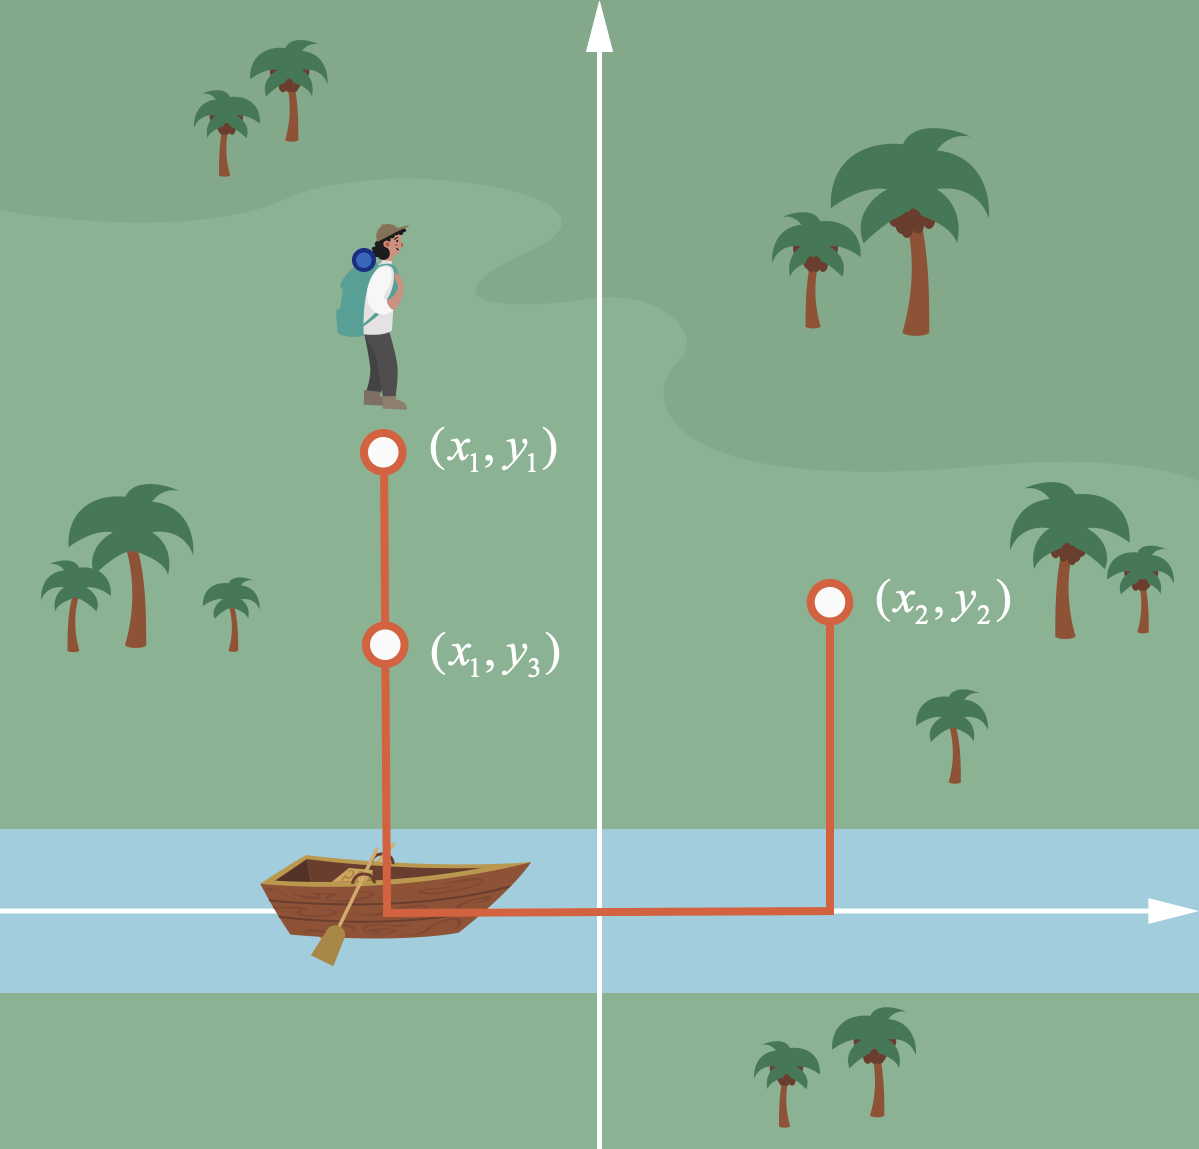
\includegraphics[width=0.5\linewidth]{jungle.png}
    \end{figure}
    \begin{proof} [Решение]
        <<Метрика Амазонки>> $\rho_\star\colon \R^2 \times \R^2 \to \R_{\geqslant 0} $, т.ч. \[
        \rho_\star((x_1, y_1), (x_2, y_2)) = \begin{cases}
            |y_1-y_2|, &x_1=x_2\\
            |y_1| + |x_1-x_2| + |y_2|, &otherwise
        \end{cases}
        \] 

        Нарисуем какие-нибудь шары. Понятно, что если $\epsilon \leq |y|$ точки $(x,y)$. То картинка будет такая:
        
        \begin{figure}[ht]
            \centering
            \begin{asy}
                size(4cm); // Size of the graph
                defaultpen(fontsize(8pt));
                
                real xmin = -1, xmax = 5, ymin = -1, ymax = 6;
                
                // Add grid lines (vertical and horizontal)
                for (real i = floor(xmin); i <= ceil(xmax); ++i) if (i != 0){
                  draw((i, ymin) -- (i, ymax), gray(0.7));  // Vertical grid lines
                }
                for (real j = floor(ymin); j <= ceil(ymax); ++j) if (j != 0){
                  draw((xmin, j) -- (xmax, j), gray(0.7));  // Horizontal grid lines
                }
                
                // Draw the axes
                xaxis(xmin-.5, xmax+.5, blue+bp,arrow=Arrow(arrowhead=DefaultHead, size=1mm)); 
                yaxis(ymin-.5, ymax+.5, arrow=Arrow(arrowhead=DefaultHead, size=1mm));
                
                
                draw((3,1)--(3,5), red);
                dot((3,3), black+3);

                dot((3,1), filltype=FillDraw(fillpen=white, drawpen=red));
                dot((3,5), filltype=FillDraw(fillpen=white, drawpen=red));
                
                draw((-.1,1)--(.1,1));
                // Label axes
                label("$x$", (xmax+0.5, 0), N);
                label("$y$", (0, ymax+0.5), E);
                label("1", (-.7, 1), UnFill(0mm));
            \end{asy}
            \caption{Шар $B_2((3,3))$ в метрическом пространстве $(\R^2, \rho_\star).$}
        \end{figure}
        \pagebreak
        Иначе же, мы сможем попасть на речку! Нарисуем парочку шаров.
    
        \begin{figure}[ht]
            \centering
            \begin{asy}
                size(4cm); // Size of the graph
                defaultpen(fontsize(8pt));
                
                real xmin = -1, xmax = 5, ymin = -3, ymax = 7;
                
                // Add grid lines (vertical and horizontal)
                for (real i = floor(xmin); i <= ceil(xmax); ++i) if (i != 0){
                  draw((i, ymin) -- (i, ymax), gray(0.7));  // Vertical grid lines
                }
                for (real j = floor(ymin); j <= ceil(ymax); ++j) if (j != 0){
                  draw((xmin, j) -- (xmax, j), gray(0.7));  // Horizontal grid lines
                }
                
                // Draw the axes
                xaxis(xmin-.5, xmax+.5, blue+bp,arrow=Arrow(arrowhead=DefaultHead, size=1mm)); 
                yaxis(ymin-.5, ymax+.5, arrow=Arrow(arrowhead=DefaultHead, size=1mm));
                
                
                draw((2,2)--(2,6), red);
                filldraw((0,0)--(2,2)--(4,0)--(2,-2)--cycle, red+opacity(0.1), red+dashed);
                draw((2,2)--(2,0)--(1.3,0)--(1.3, 1.2), dashed+deepgreen);
                dot((2,2), black+3);

                dot((2,6), filltype=FillDraw(fillpen=white, drawpen=red));
                
                draw((-.1,1)--(.1,1));
                // Label axes
                label("$x$", (xmax+0.5, 0), N);
                label("$y$", (0, ymax+0.5), E);
                label("1", (-.6, 1), UnFill(0mm));
            \end{asy}
            \hspace{2cm}
            \begin{asy}
                size(4cm); // Size of the graph
                defaultpen(fontsize(8pt));
                
                real xmin = -1, xmax = 5, ymin = -2, ymax = 4;
                
                // Add grid lines (vertical and horizontal)
                for (real i = floor(xmin); i <= ceil(xmax); ++i) if (i != 0){
                  draw((i, ymin) -- (i, ymax), gray(0.7));  // Vertical grid lines
                }
                for (real j = floor(ymin); j <= ceil(ymax); ++j) if (j != 0){
                  draw((xmin, j) -- (xmax, j), gray(0.7));  // Horizontal grid lines
                }
                
                // Draw the axes
                xaxis(xmin-.5, xmax+.5, blue+bp,arrow=Arrow(arrowhead=DefaultHead, size=1mm)); 
                yaxis(ymin-.5, ymax+.5, arrow=Arrow(arrowhead=DefaultHead, size=1mm));
                
                
                draw((3,1)--(3,3), red);
                filldraw((2,0)--(3,1)--(4,0)--(3,-1)--cycle, red+opacity(0.1), red+dashed);
                draw((3,1)--(3,0)--(3.6,0)--(3.6,0.4), dashed+deepgreen);
                dot((3,1), black+3);

                dot((3,3), filltype=FillDraw(fillpen=white, drawpen=red));
                
                draw((-.1,1)--(.1,1));
                // Label axes
                label("$x$", (xmax+0.5, 0), N);
                label("$y$", (0, ymax+0.5), E);
                label("1", (-.7, 1), UnFill(0mm));
            \end{asy}
            \caption{Щары $B_4(2,2)$ и $B_2(3,1)$ соответственно в метрическом пространстве $(\R^2, \rho_\star).$}
        \end{figure}
    \end{proof}
    \item Докажите, что в любом метрическом пространстве любой открытый шар является открытым множеством, а любой замкнутый шар является замкнутым множеством. (Обратите внимание: одного того обстоятельства, что мы назвали открытый шар открытым шаром, недостаточно, чтобы убедиться в том, что он удовлетворяет определению открытого множества.) Подсказка: необходимо явно воспользоваться неравенством треугольника.

    Приведите примеры метрических пространств и шаров в них, показывающие, что открытый шар может оказаться замкнутым множеством, а замкнутый шар может оказаться открытым множеством.
    \begin{proof}
        [Решение]
        \begin{conditions}
            \item Пусть $U_\epsilon(a)$ -- открытый шар, содержащий точку $b$. Тогда \[\rho(b, a) = \delta < \epsilon.\]
            Рассмотрим открытый шар $ U_{\epsilon-\delta}(b)$ и точку $c$ в нём. Тогда \[
            \rho(a,c) \leqslant \rho(a,b) + \rho(b,c) < \delta + \epsilon -\delta =\epsilon.
            \] 
            Значит $U_{\epsilon-\delta}(b) \subset U_\epsilon(a).$

            \item Пусть $\tilde U_\epsilon(a)$ -- замкнутый шар, а $\bar{\tilde U_\epsilon(a)}$ -- его замыкание. Понятно, что $\tilde U_\epsilon(a) \subset \bar{\tilde U_\epsilon(a)}$. Осталось доказать в обратную сторону. Пусть $\bar a \in \bar{\tilde U_\epsilon(a)}$. Тогда $\forall \delta > 0 \quad U_\delta(\bar a) \cap \tilde U_\epsilon(a) \ni c$. Тогда предположим, что $\bar a \not\in U_\epsilon(a)$ и возьмём $\delta = \rho(a,a') - \epsilon > 0$.\[
            \rho(a, \bar a) \leqslant \rho(a, c) + \rho(\bar a, c) < \epsilon + \delta = \rho(a,\bar a).
            \]
            Противоречие, значит $\bar a \in U_\epsilon(a)$.
        \end{conditions}
        В дискретной метрике любой замкнутый шар открыт и наоборот.
    \end{proof}
    \item Пусть $(X,\rho_X)$ — метрическое пространство, а $Y\subset X$. Снабдим $Y$ индуцированной метрикой $\rho_Y$, то есть положим $\rho_Y(y,y')=\rho_X(y,y')$ для любых $y,y'\in Y$.  Проверьте, что замыкание множества $A\subset Y$ относительно индуцированной метрики пространства $Y$ совпадает с $\bar A \cap Y$, где $\bar A$ — замыкание множества $A$ в пространстве $X$.
    \begin{proof}
        [Решение]
        Пусть $\tilde A = \{y \in Y\such  (\forall\epsilon > 0)(\exists \tilde y\in \tilde A) \quad \rho_Y(y, \tilde y) = \rho_X(y, \tilde y) < \epsilon\}$ -- замыкание множества $A$ относительно индуцированной метрики пространства $Y$.

        А множество $\bar A \cap Y = \{y \in Y\such (\forall \epsilon > 0)  (\exists\bar y \in \bar A) \quad \rho_X(y, \bar y) < \epsilon\}.$

        Ну и очевидно, что эти множества совпадают.
    \end{proof}
\end{tasks}
    
\end{document}